%!TEX root = ../thesis.tex

\section{地図を用いたルールベースの制御器}
従来手法と提案手法において, 教師信号として用いる地図を用いたルールベース制御器について述べる. 地図を用いたルールベース制御器は, ROS Navigation\_stack\cite{navigation:online}へ目標位置(waypoint)の指示を行うwaypoint\_nav\cite{waypoint_nav:online}を組み合わせたものである. なお, 後述するが提案手法ではwaypoint\_navの役割が増えている. ROS Navigation\_stackでは以下のような処理が行われる. 

\begin{itemize}
  \item ロボットの現在位置を推定する
  % \item 移動目標地点を決定する
  \item 移動目標地点までの経路を決定する
  \item 経路にしたがった行動をロボットに指示する
\end{itemize}

また, \figref{Fig:navigation}に示すように, 事前に作成した占有格子地図と測域センサ, オドメトリを用いて, 地図上での自己位置を確率分布をParticle\_Filterによって表現することで推定する「amcl」. 障害物認識などによる局所的, または地図全体の大域的なコスト計算, その結果に基づいた経路計画, それに従ったモータ指令を行う「move\_base」などのパッケージによって構成されている自律移動を行うためのメタパッケージである. 従来手法, 提案手法ともにモータ指令を並進速度と角速度にわけた. なお, 並進速度は一定とした.

% \vspace{5cm}

\begin{figure}[hbtp]
  \centering
 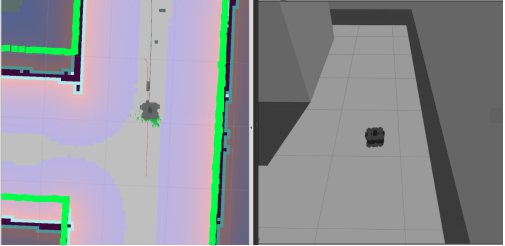
\includegraphics[keepaspectratio, scale=0.7]
      {images/navigation.png}
 \caption{A rule-based controller using a map}
 \label{Fig:navigation}
\end{figure}

% \subsubsection{etc...}
\newpage